\documentclass[9pt]{beamer}

\usepackage{appendixnumberbeamer}
\usepackage{booktabs}
\usepackage[scale=2]{ccicons}
\usepackage{pgfplots}
\usepackage{tikz}
\usepackage{graphics}

\usepgfplotslibrary{dateplot}
\pdfstringdefDisableCommands{\def\translate#1{#1}}
\geometry{paperwidth=140mm, paperheight=105mm}
\usetheme{metropolis}
\bibliographystyle{abbrv}
\setbeamertemplate{frame footer}{Lab - Mechatronics}

\usetikzlibrary{shapes, arrows}
\tikzstyle{startstop} = [rectangle, rounded corners, minimum width=2cm, minimum height=1cm, text centered, draw=black, fill=red!30]
\tikzstyle{io} = [trapezium, trapezium stretches=true, trapezium left angle=70, trapezium right angle=110, minimum width=2cm, minimum height=1cm, text centered, draw=black, fill=blue!30]
\tikzstyle{process} = [rectangle, minimum width=2cm, minimum height=1cm, text centered, text width=2cm, draw=black, fill=orange!30]
\tikzstyle{decision} = [diamond, minimum width=2cm, minimum height=1cm, text centered, draw=black, fill=green!30]
\tikzstyle{arrow} = [thick,->,>=stealth]

\title{Modelling and control of a Magnetic Levitation System}
\subtitle{Mid-project presentation}
% \date{\today}
\date{November 07, 2024}
\author{Tommaso Bocchietti 10740309 \\ Daniele Cianca 10764733 \\ Sara Orazzo 10995845}
\institute{Politecnico di Milano}
\titlegraphic{\hfill
\includegraphics[height=1.5cm]{pdf/Polimi_logo_header.pdf}}

\begin{document}

\maketitle

\begin{frame}{Agenda}

    \begin{columns}[c, onlytextwidth]

        \begin{column}{0.3\textwidth}

            \setbeamertemplate{section in toc}[sections numbered]
            \tableofcontents

        \end{column}

        \begin{column}{0.7\textwidth}

            \begin{figure}[H]
                \centering
                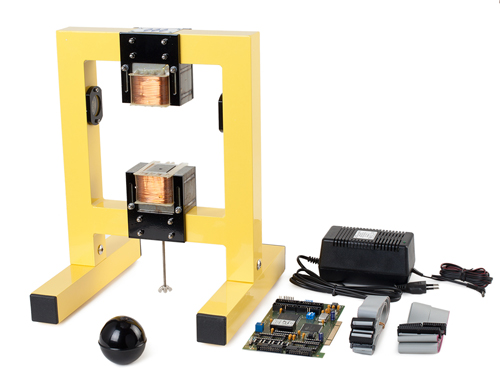
\includegraphics[width=0.8\textwidth]{img/maglev_and_components.jpg}
                \caption{Magnetic Levitation System and its components}
            \end{figure}

        \end{column}

    \end{columns}

\end{frame}

% \begin{frame}{Title of the frame}

    % Content of the frame

    % Some simple text with formulas
    My beautiful formula ($y = mx + q$) and some text.

    % Two columns template
    \begin{columns}[c, onlytextwidth]

        \begin{column}{0.3\textwidth}

            A simple list:

            \begin{itemize}
                \item First item
                \item Second item
                \item Third item
            \end{itemize}

        \end{column}

        \begin{column}{0.7\textwidth}

            % A big equation
            \begin{equation}
                \begin{aligned}
                    \dot{x} & = Ax + Bu \\
                    y       & = Cx + Du
                \end{aligned}
            \end{equation}

        \end{column}

    \end{columns}

\end{frame}
\section{Project objectives}

\begin{frame}{Magnetic Levitation System (MLS)}

    Magnetic Levitation System (MLS), also known as MagLev, is a highly nonlinear system that can be used to study control strategies.
    It's composed of two electromagnets that are driven in voltage to generate a magnetic field in order levitates a metallic ball sitting in between them.

    \vspace{9pt}

    Project objectives can be divided as follows.

    \begin{columns}[c, onlytextwidth]

        \begin{column}{0.5\textwidth}

            Modelling:

            \begin{itemize}
                \item Literature review
                \item Equations of motion
                \item Parameters identification
            \end{itemize}

        \end{column}

        \begin{column}{0.5\textwidth}

            Controlling:

            \begin{itemize}
                \item Simulink model
                \item Linear controllers
                \item Nonlinear controllers
            \end{itemize}

        \end{column}

    \end{columns}

\end{frame}
\section{Modelling}

\begin{frame}{Scheme of MLS system}

    Even if MLS is composed of two coils, for the aim of this work we have chosen to focus on the \textbf{single coil configuration}, considering only the upper one.

    \begin{figure}[H]

        \begin{minipage}{0.40\textwidth}

            \centering

            \begin{tikzpicture}[european voltages]

                \def\radius{0.3}

                % Upper circuit
                \draw (-3, 3.5) node [right] {$+$}
                to [short] ++(0, -1)
                to [R, l^=$R$, resistors/zigs=6] ++(2, 0)
                to [variable cute inductor, i>^=$\dot{q}$, l=$L$] ++(2, 0)
                to [short] ++(0, +1) node [right] {$-$};

                % Reference system
                \draw[|->] (-1.0, +2.5) -- ++(0, -2.5 + \radius) node[left] {$z$, $\dot{z}$, $\ddot{z}$};

                % Ball
                \filldraw[fill=gray, draw=black] (0, 0) circle (\radius);

                % Upward forces
                \draw[thick, ->] (-0.1, +\radius) -- ++(0, +1.5) node[right] {$F_{\text{em}}$};
                \draw[thick, ->] (+0.0, +\radius) -- ++(0, +1.0) node[right] {$F_{\text{in}}$};
                \draw[thick, ->] (+0.1, +\radius) -- ++(0, +0.5) node[right] {$F_{\text{d}}$};

                % Downward forces
                \draw[thick, ->] (+0.0, -\radius) -- ++(0, -0.5) node[right] {$F_{\text{g}}$};

            \end{tikzpicture}

        \end{minipage}
        %
        \hfill
        %
        \begin{minipage}{0.55\textwidth}

            \begin{table}
                \centering

                \begin{tabular}{|c|l|}
                    \hline
                    \textbf{Name}   & \textbf{Description}  \\
                    \hline
                    $F_{\text{g}}$  & Gravitational force   \\
                    $F_{\text{in}}$ & Inertial force        \\
                    $F_{\text{d}}$  & Drag force            \\
                    $F_{\text{em}}$ & Electromagnetic force \\
                    \hline
                \end{tabular}

            \end{table}

        \end{minipage}

        \label{fig:MLS_scheme}

    \end{figure}

\end{frame}



\begin{frame}{Lagrange equation}

    To derive the \textbf{equations of motion}, we started from the Lagrange equation of the system:

    \begin{equation}
        \frac{d}{dt} \left( \frac{\partial \mathcal{T}}{\partial \dot{\mathbf{u}}} \right) - \frac{\partial \mathcal{T}}{\partial \mathbf{u}} + \frac{\partial \mathcal{D}}{\partial \dot{\mathbf{u}}} + \frac{\partial \mathcal{U}}{\partial \mathbf{u}} = \mathcal{Q}
        \text{, where }
        \mathbf{u} = \begin{bmatrix} z \\ q \end{bmatrix}
        \label{eq:lagrange_equation}
    \end{equation}

    The energy terms are defined as follows:

    \begin{equation}
        \begin{aligned}
            \mathcal{T} & = \frac{1}{2} m \dot{z}^2 + \frac{1}{2} L(z, \dot{q}) \dot{q}^2                                                       \\
            \mathcal{D} & = \int_{\dot{z}(\cdot)} \frac{1}{2} C_d A \rho \dot{z}^2 d\dot{z} + \int_{\dot{q}(\cdot)} R(\dot{q}) \dot{q} d\dot{q} \\
            \mathcal{U} & = -m g z - q V                                                                                                        \\
            \mathcal{Q} & = 0
        \end{aligned}
    \end{equation}

\end{frame}



\begin{frame}{Electrical components model}

    Based on experimental data, we have proposed a model for both the resistance and the coil inductance:

    \begin{equation}
        \begin{aligned}
            R & = R(I) = R_{0}                                                          \\
            L & = L(z, I) = L_{0} + L_{z} e^{-a_{z} z} + L_{I} \arctan(a_{I} I - b_{I})
        \end{aligned}
        \label{eq:model_for_inductance}
    \end{equation}

    The first and second derivatives with respect to ball position and current are:

    \begin{equation}
        \begin{aligned}
            \frac{\partial L}{\partial z}     & = -a_{z} L_{z} e^{-a_{z} z}  \\
            \frac{\partial^2 L}{\partial z^2} & = a_{z}^2 L_{z} e^{-a_{z} z}
        \end{aligned}
        \qquad
        \begin{aligned}
            \frac{\partial L}{\partial I}     & = \frac{L_{I} a_{I}}{1 + (a_{I} I - b_{I})^2}                            \\
            \frac{\partial^2 L}{\partial I^2} & = -2 \frac{L_{I} a_{I}^2 (a_{I} I - b_{I})}{(1 + (a_{I} I - b_{I})^2)^2}
        \end{aligned}
        \label{eq:model_for_inductance_derivatives}
    \end{equation}

\end{frame}



\begin{frame}{Model approximations}

    In order to simplify the model, some approximations have been considered:

    \begin{equation}
        \begin{cases}
            \frac{\partial L}{\partial I}     & \approx 0 \\
            \frac{\partial^2 L}{\partial I^2} & \approx 0 \\
            \dot{z}                           & \approx 0
        \end{cases}
        \label{eq:model_reduction_conditions}
    \end{equation}

    Notice that, from successive analysis, these approximations have proven (at least in the range of interest) to be valid.

\end{frame}



\begin{frame}{Equations of motion}

    By applying approximations of Equation (\ref{eq:model_reduction_conditions}) to the Lagrange equation (\ref{eq:lagrange_equation}), we have obtained the following equations of motion:

    \begin{equation}
        \begin{cases}
            \dot{z} = v                                                                         \\
            \dot{v} = m^{-1} \left(\frac{1}{2} \frac{\partial L}{\partial z} I^2 + m g  \right) \\
            \dot{I} = L^{-1} \left(- R I + V \right)
        \end{cases}
        \label{eq:equations_of_motion_single_coil}
    \end{equation}

    Model non-linearities are hidden in all the terms relative to the inductance $L$ and its derivatives.

    \vspace{9pt}

    Despite the applied approximations, the set of Equations (\ref{eq:equations_of_motion_single_coil}) is still \textbf{able to capture the main dynamics of the system}.

\end{frame}

\section{Controlling}


\section{Future work}

\begin{frame}{What we want to achieve?}

\end{frame}

\appendix

\begin{frame}[allowframebreaks]{References}
    \nocite{*}
    \bibliography{references}
\end{frame}

\begin{frame}[standout]
    Questions?
\end{frame}

\begin{frame}[standout]
    Thank you!
\end{frame}

\end{document}